\textbf{1--3. Fixed-free bar.} The left end is fixed and the right end has zero axial force.
\begin{figure}[H]
\centering
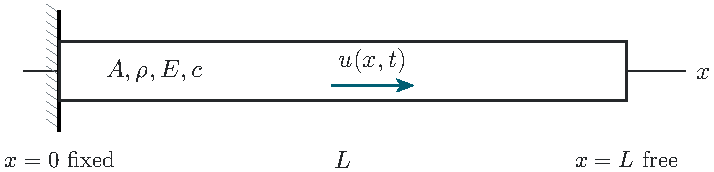
\includegraphics[width=0.78\linewidth]{figures/generated/solutions/C11-bar.pdf}
\caption{Axial vibration of a fixed-free bar.}
\end{figure}
The boundary conditions are $u(0,t)=0$ and $\sigma(L,t)=E u_x(L,t)=0$. Substitution of $u=Ue^{-i\omega t}$ and $U=C_1\sin\gamma x+C_2\cos\gamma x$ gives
\[
U(0)=C_2=0,\qquad
U'(L)=\gamma\left[C_1\cos(\gamma L)-C_2\sin(\gamma L)\right]=0.
\]
For $\gamma>0$, the fixed condition removes $C_2$ and the free condition becomes $C_1\cos(\gamma L)=0$. The trivial choice $C_1=0$ gives zero motion. For nonzero amplitude, $\cos z=0$ with $z=\gamma L$. Its successive positive roots are odd multiples of $\pi/2$, so
\[
z_j=\frac{(2j-1)\pi}{2},\quad
\gamma_j=\frac{(2j-1)\pi}{2L},\quad
\omega_j=\frac{(2j-1)\pi c}{2L},\quad
f_j=\frac{(2j-1)c}{4L}.
\]
With $j=1,2,\ldots$ and $\lambda=2\pi/\gamma$, the wavelengths satisfy
\[
\lambda_j=\frac{4L}{2j-1},\qquad L=(2j-1)\frac{\lambda_j}{4}.
\]
The fundamental is $f_1=c/(4L)$. The overtones occur at the higher odd multiples $3f_1,5f_1,\ldots$. Setting $C_1=1$ gives
\[
\boxed{U_j(x)=\sin\frac{(2j-1)\pi x}{2L},\qquad
\frac{2}{L}\int_0^L U_jU_k\,dx=\delta_{jk},\qquad
\Sigma_j(x)=E\gamma_j\cos(\gamma_j x).}
\]
The results follow course-note axial vibration section 3.2, PDF pages 226--230.

The displacement vanishes at the fixed end and reaches an antinode at the free end. The fundamental fits one quarter-wavelength in the bar, while successive modes add half-wavelengths. Differentiation gives $\Sigma_j=EU_j'$, which vanishes at the free end because $\cos(\gamma_j L)=0$. The integral of $U_j^2$ over the bar is $L/2$, and distinct modes have zero cross-integral, establishing the stated orthonormality relation.
